\documentclass[Main.tex]{subfiles}
\begin{document}
%========================================================================== %
\setcounter{tocdepth}{1}

\begin{verbatim}


A: Introduction to LME Models, Fitting LME Models to MCS Data

In this section, we introduce the LME model, discusss how it can be applied to MCS problems, and how it is desirable in the case of replicate measurements, giving some examples from previous work (i.e. Carstensen et Al, Lai \& Shaio, and Roy)
Further to that, there will be a discussion on fitting various types LME models using freely available software. To fully understand the complexities, a comparison of the nlme and LME4 R Packages is required.
While the MCS problem is conventionally poised in the context of two methods of measurements, LME models allow for a straightforward analysis that looks at several methods of measurement simulataneously, specifically looking at inter-method bias.


B: Residual Analysis for LME, Applications to MCS Data

This short section will look at residual analysis for LME models. The underlying assumptions for LME models are similar to those of classical linear mdoels. There are two key techniques: a residual plot and the normal probability plot. Using the nlme package it is possible to create plots specific to each method. This is useful in determine which methods `disagree` with the rest.
Analysis of the residuals would determine if the methods of measurement disagree systematically, or whether or not erroneous measurements associated with a subset of the cases are the cause of disagreement.
Erroneous measurements are incorrect measurements that indicate disagreement between methods that would otherwise be in agreement.


C: Case Deletion Diagnostics for LME Data: Cooks Distance, DFBetas
In this section we introduce influence analysis and case deletion diagnosics. A full overview of the topic will be provided although there are specific tools that are useful in the case of MCS problems.
A discussion of how leave-k-out diagnostics would work in the context of MCS problems is required.

D: Using DFBETAs to assess agreement
Suppose an LME model was formulated to model agreement for various (i.e. 2or more) methods of measurement, with replicate measurements. If the methods are to be agreement, the DFBetas for each case would be the same for both metods.
As such, agreement between any two methods can be determined by a simple scatterplot of the DFBetas. 
IF the points align along the line of equality, then both methods can be said to be in agreement. 
If they appear not to be agreement, asubsequent analysis using a technique proposed by Roy(2009) can be used to identify the specific cause for this lack of agreement.

The Pearson Correlation coefficient of the DFBetas can be used in conjection with this analysis.

E: Using Roy's Test to Identify cause of Lack of agreement

Barnhard specifies three conditions for method of measurement that are required for two methods of measurement to be considered in agreement.

  i) No Significant Inter-method bias
  ii) No significant Difference in Within-Subject Variance
  iii) No significant Difference in Within-Subject Variance 

F: Using Roy's Model to Compute LoAs and CR 

In this short section, a demonstration of how Roy's technique can be used to compute two common MCS metrics: Limits of Agreement and the Coefficient of Repeatabilty.

G: Model Diagnostics for Roy's Models

Further to previous work, this secton revisits case-deletion and residual diagnostics, and explores how approaches devised by Galecki and Burzykowski can be used to appraise the model.

H: Permutation and Power Tests  


\endv{verbatim}
%================================================%
\tableofcontents
	
\chapter{Fitting LME Models}
%\subsection{Overview of R implementations}
Further to previous material, an appraisal of the current state of development for statistical software for fitting for LME models, particularly for \texttt{nlme} and \texttt{lme4} fitted models.

%======================%
% lme4 and influence.ME

The \textbf{lme4} pacakge is used to fit linear and generalized linear mixed-effects models in the R environment.
The \textbf{lme4} package is also under active development, under the leadership of Ben Bolker (McMaster Uni., Canada).


Crucially, a review of internet resources indicates that almost all of the progress in this regard has been done for \texttt{lme4} fitted models, specifically the \textit{Influence.ME} \texttt{R} package. (Nieuwenhuis et al 2014)
Conversely there is very little for \texttt{nlme} models. One would immediately look at the current development workflow for both packages.

%======================%
% Douglas Bates

As an aside, Douglas Bates was arguably the most prominent \texttt{R} developer working in the LME area. 
However Bates has now prioritised the development of LME models in another computing environment , i.e Julia. 
% The current version of this is XXXX

%======================%
% nlme

With regards to \texttt{nlme}, the package is now maintained by the \texttt{R} core development team. The most recent major text is by Galecki \& Burzykowski, who have published \textit{ Linear Mixed Effects Models using \texttt{R}. }
Also, the accompanying \texttt{R} package, nlmeU package is under current development, with a version being released $0.70-3$.


\section{Fitting Models with nlme R package}

%-------------------------------------------------------------------------------------------------------------------------------------%
\section{Fitting Models with the LME4 R package}
Maximum likelihood or restricted maximum likelihood (REML) estimates of the parameters in linear mixed-effects models can be determined using the \texttt{lmer} function in the lme4 package for R. As for most model-fitting functions in R, the model is described in an \texttt{lmer} call by a formula, in this case including both fixed- and random-effects terms. 

The formula and data together determine a numerical representation of the model from which the profiled deviance or the profiled REML criterion can be evaluated as a function of some of the model parameters. The appropriate criterion is optimized, using one of the constrained optimization functions in \texttt{R}, to provide the parameter estimates. We describe the structure of the model, the steps in evaluating the profiled deviance or REML criterion, and the structure of classes or types that represents such a model. 

Sufficient detail is included to allow specialization of these structures by users who wish to write functions to fit specialized linear mixed models, such as models incorporating pedigrees or smoothing splines, that are not easily expressible in the formula language used by lmer.


\begin{description}
	\item[\texttt{y}] : Response variable
	\item[\texttt{method}] : Method of Measurement
	\item[\texttt{subject}] : Subject
	\item[\texttt{MCSdata}] 
\end{description}
\begin{framed}
	\begin{verbatim}
	library(lme4)
	
	MCS.lme4 <- lmer(y ~ method-1 + (1|subject) , data=MCSdata)
	\end{verbatim}
\end{framed}
\newpage

%=====================%
\subsection{Important Consideration for MCS}

The key issue is that \texttt{nlme} allows for the particular specification of Roy's Model, specifically direct specification of the VC matrices for within subject and between subject residuals.

The \texttt{lme4} package does not allow for Roy's Model, for reasons that will identified shortly.
To advance the ideas that eminate from Roys' paper, one is required to use the \texttt{nlme} context. However, to take advantage of the infrastructure already provided for \texttt{lme4} models, one may change the research question away from that of Roy's paper. 
To this end, an exploration of what textbf{influence.ME} can accomplished is merited.





%============================================================%
\newpage
\section{Diagnostic Tools for the nlme package}


With the nlme package, the generic function \texttt{lme()} fits a linear mixed-effects model in the formulation described in Laird and Ware (1982) but allowing for nested random effects. 

The within-group errors are allowed to be correlated and/or have unequal variances, which is very important in fitting the models for Roy's Tests

The nlme package has a limited set of diagnostic tools that can be used to assess the model fit. A review of the package manual is sufficient to get a sense of the package's capability in that regard.

\begin{description}
	\item[residuals.lme] 
	The residuals at level $i$ are obtained by subtracting the fitted levels at that level from the response
	vector (and dividing by the estimated within-group standard error, if \texttt{type="pearson")}. The fitted
	values at level $i$ are obtained by adding together the population fitted values (based only on the
	fixed effects estimates) and the estimated contributions of the random effects to the fitted values at
	grouping levels less or equal to $i$.
\end{description}


\chapter{Residual Analysis}
A residual is the difference between an observed quantity and its estimated or predicted value. In LME models, there are two types of residuals, marginal residuals and conditional residuals. A marginal residual is the difference between the observed data and the estimated marginal mean. A conditional residual is the difference between the observed data and the predicted value of the observation. In a model without random effects, both sets of residuals coincide.

\section{Residual diagnostics} %1.3
\subsection{Introduction to Residual Analysis}
%A residual is the difference between an observed quantity and its estimated or predicted value. 
Residual analysis is a widely used model validation technique. A residual is simply the difference between an observed value and the corresponding fitted value, as predicted by the model. The rationale is that, if the model is properly fitted to the model, then the residuals would approximate the random errors that one should expect; if the residuals behave randomly, with no discernible trend. If some sort of non-random trend is evident in the model, then the model can be considered to be poorly fitted.

For classical linear models, residual diagnostics are typically implemented as a plot of the observed residuals and the predicted values. A visual inspection for the presence of trends inform the analyst on the validity of distributional assumptions, and to detect outliers and influential observations. Statistical software environments, such as the \texttt{R} programming language, provides a suite of tests and graphical procedures for appraising a fitted linear model, with several 
of these procedures analysing the model residuals.

However, for LME models the matter of residual is more complex, both from a theoretical point of view and from the practical matter of implementing a comprehensive analysis using statistical software. As the LME model can be tailored to the needs of the particular research question, the rationale behind the model appraisal must follow accordingly.


%===================================================================================================%
\subsection{Residuals in the Blood Data Example}
The fitted model used in the Blood data example, \texttt{JS.roy1}, was fitted using the \texttt{lme()} function from the nlme package, and as such, is stored as an \texttt{lme} object. The \texttt{residual} functions extracts residuals of a fitted LME model, depending on the type of residual required.

For an lme object, the residuals at level $i$ are obtained by subtracting the fitted levels at that level from the response vector (and dividing by the estimated within-group standard error, if \texttt{type="pearson"}).The Pearson residual is the raw residual divided by the square root of the variance function (here, the Within-group standard error for both methods, 6.11 and 9.11 respectively). The fitted values at level $i$ are obtained by adding together the population fitted values (based only on the fixed effects estimates) and the estimated contributions of the random effects to the fitted values at grouping levels less or equal to $i$.

\begin{description}
	\item["\texttt{response}"]: the “raw” residuals (\textit{observed - fitted}) are used. This is the default option.
	\item["\texttt{pearson}"]: the standardized residuals (raw residuals divided by the corresponding standard errors) are used; 
	\item["\texttt{normalized}"]: the normalized residuals (standardized residuals pre-multiplied by the inverse square-root factor of the estimated error correlation matrix) are used.
\end{description}

\begin{framed}
	\begin{verbatim}
	data.frame( response = resid(JS.roy1, type = "response"), 
	pearson  = resid(JS.roy1, type = "pearson"), 
	normalized = resid(JS.roy1, type = "normalized") )
	\end{verbatim}
\end{framed}

\begin{verbatim}
response      pearson    normalized
1    -4.65805902 -0.761587227 -0.7615872269
2    -0.88701342 -0.145025661  0.0776238081
3    -5.16580898 -0.844603753 -0.8446037530
4     2.29041830  0.374480726  0.6450898404
5     7.87508366  1.287567009  1.2875670086
6    -6.57048659 -1.074266908 -1.5090772378
...........................................
\end{verbatim}
For the $J$ observations, the variance is 6.116252 whereas for the $S$ observations, the denominator is 9.118144. (with the expected ratio of  1.490806)


\begin{framed}
	\begin{verbatim}
	> pearson %>%
	+   as.numeric %>% 
	+   matrix(nrow=85) %>%
	+   round(4) 
	[,1]    [,2]    [,3]    [,4]    [,5]    [,6]
	[1,] -0.7616  0.2194  0.3829 -0.2983  0.3597 -0.0790
	[2,] -0.1450  0.1820 -0.1450 -0.5014  0.1567  0.2663
	[3,] -0.8446  0.4634  0.1364 -0.1630 -0.2727  0.1660
	[4,]  0.3745 -0.2795 -0.2795 -0.2658 -0.2658  0.6115
	[5,]  1.2876 -0.6744 -0.6744  0.8935 -0.0935 -0.8612
	[6,] -1.0743  1.8687 -0.7473 -0.0383  0.2908 -0.3673
	...........................................
	
	\end{verbatim}
\end{framed}

We can plot the residuals against the fitted values, to assess the assumption of constant variance. 
\begin{framed}
	\begin{verbatim}
	# standardized residuals versus fitted values 
	plot(JS.roy1, resid(., type = "pearson") ~ fitted(.) , 
	abline = 0, id = 0.05)
	\end{verbatim}
\end{framed}
\begin{figure}[h!]
	\centering
	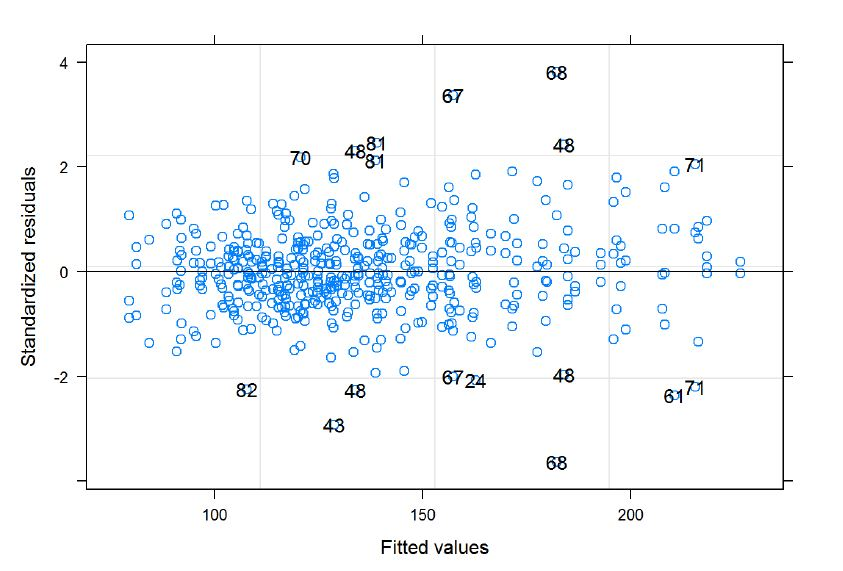
\includegraphics[width=0.9\linewidth]{images/Residuals-JS-Roy}
	\caption{}
	\label{fig:Residuals-JS-Roy}
\end{figure}

%===================================================================================================%
\subsection{Normality of Residuals in the Blood Data Example}
LME models assume that the residuals of the model are normally distributed.  The residuals can be divided according to groups according to the method of measurement. In the following examples, we seperately assess normality the \textit{J} method residuals (the first 255 residuals) and \textit{S} method residuals (the remaining 255). Importantly the residuals from the \textit{J} method are normally distributed, but there is non-normality of the residuals according to the \textit{S} method.
\begin{framed}
	\begin{verbatim}
	> shapiro.test(resid(JS.roy1)[1:255])
	
	Shapiro-Wilk normality test
	
	data:  resid(JS.roy1)[1:255]
	W = 0.9931, p-value = 0.2852
	\end{verbatim}
\end{framed}

\begin{framed}
	\begin{verbatim}
	> shapiro.test(resid(JS.roy1)[256:510])
	
	Shapiro-Wilk normality test
	
	data:  resid(JS.roy1)[256:510]
	W = 0.9395, p-value = 9.503e-09
	\end{verbatim}
\end{framed}
\begin{figure}[h!]
	\centering
	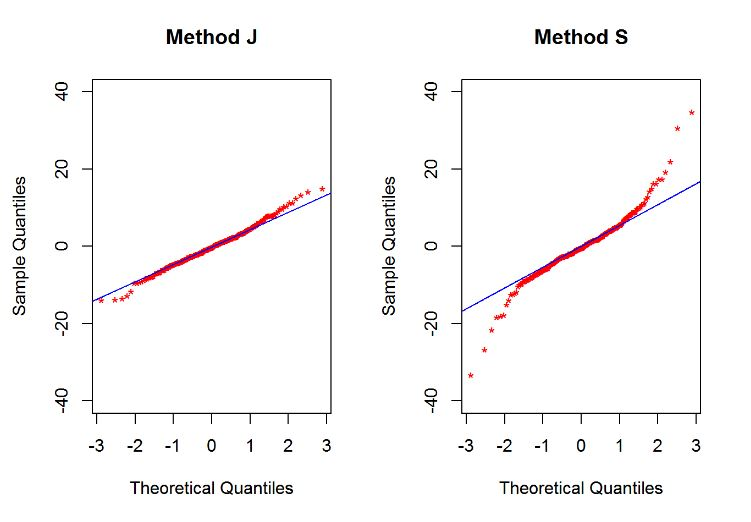
\includegraphics[width=0.9\linewidth]{images/Resid-newplot2}
	\caption{}
	\label{fig:Resid-newplot2}
\end{figure}

\newpage


\subsection{Conditional and Marginal Residuals}
A residual is the difference between an observed quantity and its estimated or predicted value. For LME models, \citet{schab} describes two types of residuals, marginal residuals and conditional residuals. 

\begin{itemize}
	\item A marginal residual is the difference between the observed data and the estimated (marginal) mean, $r_{mi} = y_i - x_0^{\prime} \hat{b}$
	\item A conditional residual is the difference between the observed data and the predicted value of the observation,
	$r_{ci} = y_i - x_i^{\prime} \hat{b} - z_i^{\prime} \hat{\gamma}$	
\end{itemize} 
In a model without random effects, both sets of
residuals coincide \citep{schab} . We shall revert to this matter in due course.



%\subsection{Marginal and Conditional Residuals}




In linear mixed effects models, diagnostic techniques may consider `conditional' residuals. A conditional residual is the difference between an observed value $y_{i}$ and the conditional predicted value $\hat{y}_{i} $.

\[ \hat{\epsilon}_{i} = y_{i} - \hat{y}_{i} = y_{i} - ( X_{i}\hat{\beta} + Z_{i}\hat{b}_{i}) \]

However, using conditional residuals for diagnostics presents difficulties, as they tend to be correlated and their variances may be different for different subgroups, which can lead to erroneous conclusions.

%========================================================%

\newpage
\subsection{Residual Analysis for MCS}

\begin{figure}[h!]
	\centering
	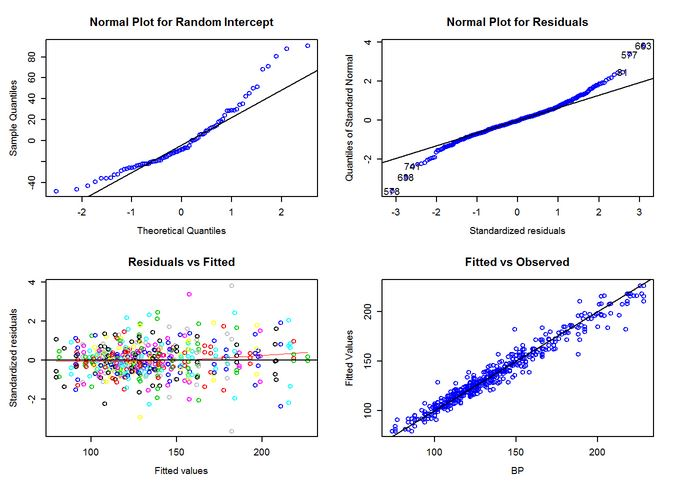
\includegraphics[width=0.9\linewidth]{images/ResidPlot}
	\caption{}
	\label{fig:ResidPlot}
\end{figure}


\subsection{PRESS Residuals and PRESS Statistic}
% % - Wikipedia
In statistics, the predicted residual sum of squares (PRESS) statistic is a form of cross-validation used in regression analysis to provide a summary measure of the fit of a model to a sample of observations that were not themselves used to estimate the model. It is calculated as the sums of squares of the prediction residuals for those observations.

A fitted model having been produced, each observation in turn is removed and the model is refitted using the remaining observations. The out-of-sample predicted value is calculated for the omitted observation in each case, and the PRESS statistic is calculated as the sum of the squares of all the resulting prediction errors:[4]
\[\mbox{PRESS} =\sum_{i=1}^n (y_i - \hat{y}_{i, -i})^2 \]
Given this procedure, the PRESS statistic can be calculated for a number of candidate model structures for the same dataset, with the lowest values of PRESS indicating the best structures. Models that are over-parameterised (over-fitted) would tend to give small residuals for observations included in the model-fitting but large residuals for observations that are excluded.

% % - http://support.sas.com/documentation/cdl/en/statug/63347/HTML/default/viewer.htm#statug_mixed_sect027.htm
An (unconditional) predicted value is $\hat{y}_i = x^{\prime}_i \boldsymbol{\hat{\beta}}$, where 
the vector $x_i$ is the $i$th row of $\boldsymbol{X}$. For an \texttt{lme} object, such as our fitted model \texttt{JS.roy1}, the predicted values for each subject can be determined using the \texttt{coef.lme} function.
\begin{framed}
	\begin{verbatim}
	> JS.roy1 %>% coef %>% head(5)
	methodJ   methodS
	74     84.31724  91.08404
	36     91.54994  97.05548
	3      81.16581  96.48653
	62     92.09493  90.89073
	31     88.41411 103.38802
	\end{verbatim}
\end{framed}



The (raw) residual is given as $\varepsilon_i = y_i - \hat{y}_i$. The PRESS residual is
similarly constructed, using the predicted value for observation $i$ with a model fitted from reduced data.
\[ \varepsilon_{i(U)} = y_i - x^{\prime}_i \boldsymbol{\hat{\beta}}_{(U)} \]
The PRESS statistic is the sum of the squared PRESS residuals:
\[ PRESS = \sum \varepsilon^2_{i(U)} \]
where the sum is over the observations in $\boldsymbol{U}$.


%---------------------------------------------------------------------------%
\newpage

Pinheiro and Bates provide some insight into how to compute and interpret model diagnostic plots for lme models. Unfortunately this aspect of LME theory is not as expansive as the corresponding body of work for Linear Models.
\section{Checking the Assumption by Method}


\subsection{Residual Analysis}


\textbf{qqnorm.lme}
% {nlme}	R Documentation
Normal Plot of Residuals or Random Effects from an lme Object

Description

Diagnostic plots for assessing the normality of residuals and random effects in the linear mixed-effects fit are obtained. 
The form argument gives considerable flexibility in the type of plot specification. 
A conditioning expression (on the right side of a | operator) always implies that different panels are used 
for each level of the conditioning factor, according to a Trellis display.

%============================================================================== %

%====================================================================%
\subsubsection{Residuals plots}

lme allows to plot the residuals in the following ways:

\begin{framed}
	\begin{verbatim}
	res_lme=residuals(model_lme)
	plot(res_lme)
	qqnorm(res_lme)
	qqline(res_lme)
	plot(model_lme)
	\end{verbatim}
\end{framed}

%==============================================================%


\subsection{Diagnostic Plots for LME models}



When the \texttt{plot} function calls the model object, the residual plot is produced.





\begin{framed}
	\begin{verbatim}
	plot(JS.roy1, which=c(1) )
	\end{verbatim}
\end{framed}


\begin{figure}[h!]
	\centering
	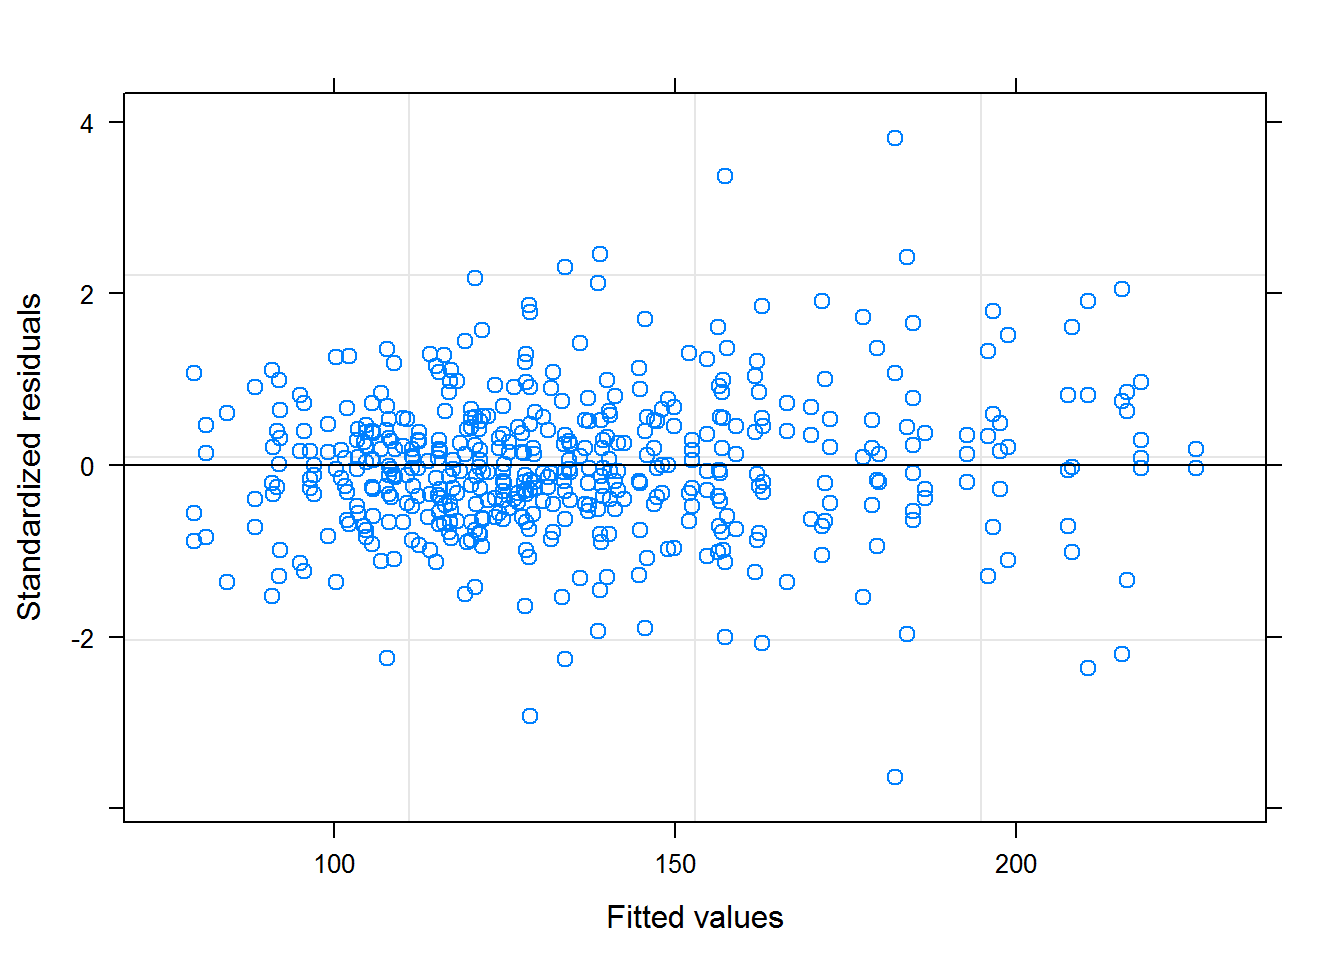
\includegraphics[width=0.9\linewidth]{images/ResidPlot1}
	\caption{}
	\label{fig:ResidPlot1}
\end{figure}
LME models assume that the residuals of the model are normally distributed. A Normal probability plot can be constructed to check this assumption. Commonly used \texttt{R} commands can be used to construct the plot.
\newpage

\begin{framed}
	\begin{verbatim}
	qqnorm(resid(JS.roy1),pch="*",col="red")
	qqline(resid(JS.roy1),col="blue")
	\end{verbatim}
\end{framed}




\begin{figure}[h!]
	\centering
	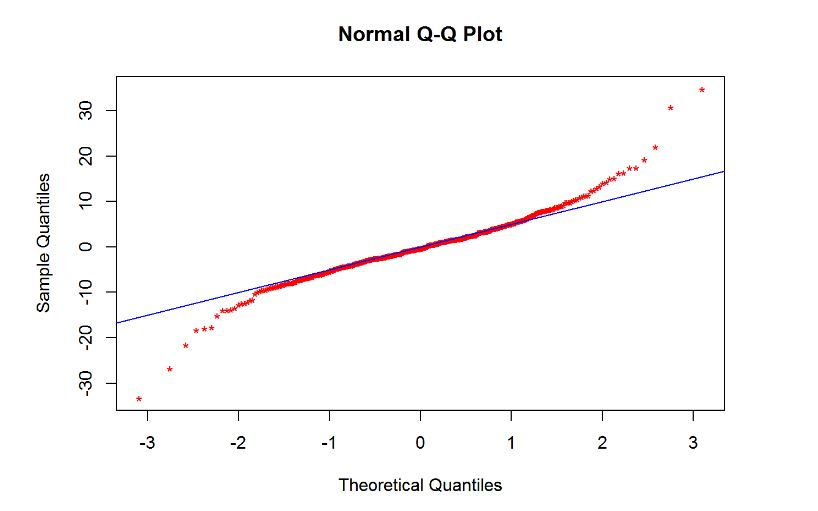
\includegraphics[width=0.7\linewidth]{images/Resid-newplot}
	\caption{}
	\label{fig:Resid-newplot}
\end{figure}

\begin{framed}
	\begin{verbatim}
	table(dat$method[1:255])
	## 
	##   J   S 
	## 255   0
	table(dat$method[256:510])
	## 
	##   J   S 
	##   0 255
	\end{verbatim}	
\end{framed}
%==================================================================================%
\newpage
\begin{framed}
\begin{verbatim}
plot(roy.NLME, resid(., type = "p") ~ fitted(.) | method, 
   abline = 0, id=.05)
\end{verbatim}
\end{framed}
\begin{figure}
\centering
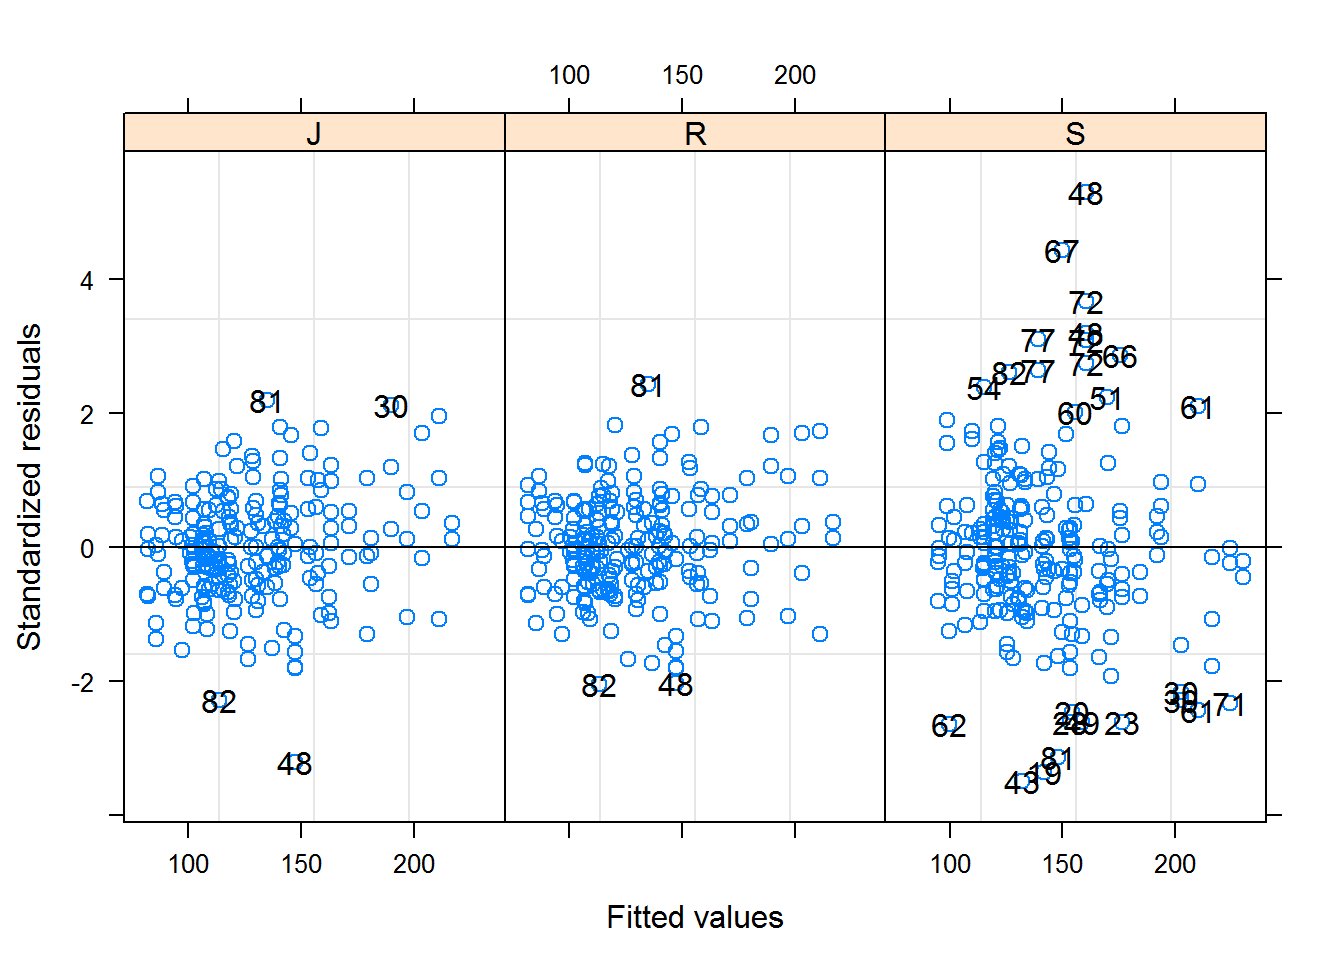
\includegraphics[width=0.9\linewidth]{images/bloodnlmeResidPlot2}
\caption{}
\label{fig:blood}
\end{figure}


\subsubsection{Cooks distance- Predict means thing here}
Cook's Distance is a model diagnostic measure of an observation that is a measure of aggregate impact of each observation on the group of regression coefficients. Observations, or sets of observations, that have high Cook's distance usually have high resdiauls. We will revisit Cook's distance fully in due cource.

Cook's Distance is a good measure of the influence of an observation that is a measure of aggregate impact of each observation on the group of regression coefficients, as well as the group of fitted values.

The \texttt{CookD} fucntion , from the predictmeans R package, produces Cook’s distance plots for an LME model 
 (predictmeans)



\begin{framed}
\begin{verbatim}
library(predictMeans)
CookD(model, group=method, plot=TRUE, idn=5, newwd=FALSE)
\end{verbatim}
\end{framed}


\begin{verbatim}
## Cook's Distance

\end{verbatim}

The particular cases that we will omit for the subsequent analysis are subjects 68,78 and 80.

\subsubsection{Reduced Data Set}
It is important to determine if a specific group of cases or subjects give rise to the lack of agreement in the methods. If one were to examine fitted model if these cases were removed.

\begin{framed}
\begin{verbatim}

blood.red <- blood[!(blood$subject %in% c(68,78,80)),]
dim(blood.red)
# 27 observations should be removed.

roy.NLME.red <-lme(BP ~ method-1 , random=~1|subject,data = blood.red)
plot(roy.NLME.red, resid(., type = "p") ~ fitted(.) | method, abline = 0, id=.05)
\end{verbatim}
\end{framed}

In this instance, we conclude that there is a systemic diagreement between method S and the other two methods, and that lack of agreement can not be sourced to a handful of cases.
\begin{figure}[h!]
	\centering
	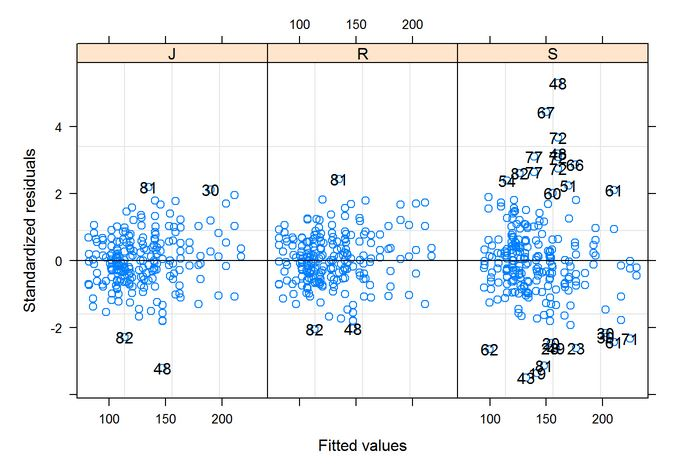
\includegraphics[width=0.7\linewidth]{images/bloodnlmeResidPlot2B}
\end{figure}


\newpage


\subsection{Residual Plots}
A residual plot is a graph that shows the residuals on the vertical axis and the independent variable on the horizontal axis. If the points in a residual plot are randomly dispersed around the horizontal axis, a linear regression model is appropriate for the data; otherwise, a non-linear model is more appropriate.

\begin{framed}
	\begin{verbatim}
	par(mfrow=c(1,2))
	qqnorm((resid(JS.roy1)[1:255]),
	pch="*",col="red",
	ylim=c(-40,40),
	main="Method J")
	qqline(resid(JS.roy1)[1:255],col="blue")
	qqnorm((resid(JS.roy1)[256:510]),
	pch="*",col="red",
	ylim=c(-40,40),
	main="Method S")
	qqline(resid(JS.roy1)[256:510],col="blue")
	par(mfrow=c(1,1))
	\end{verbatim}	
\end{framed}


\begin{figure}[h!]
	\centering
	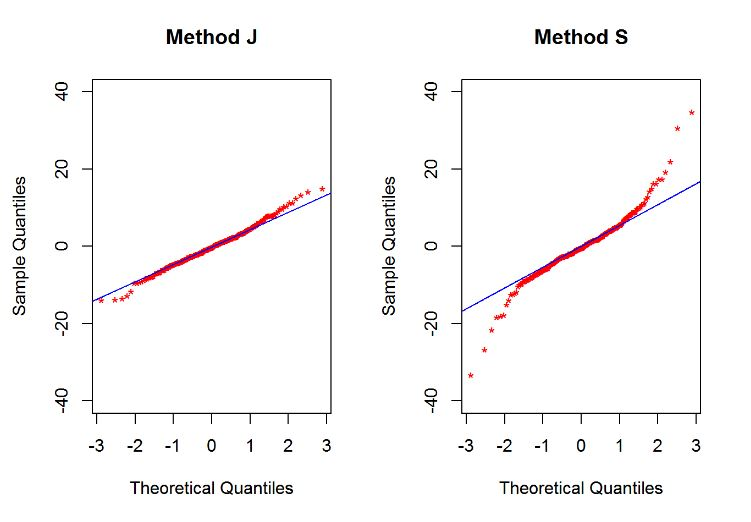
\includegraphics[width=1.1\linewidth]{images/Resid-newplot2}
	\caption{}
	\label{fig:Resid-newplot2}
\end{figure}


\begin{figure}[h!]
	\centering
	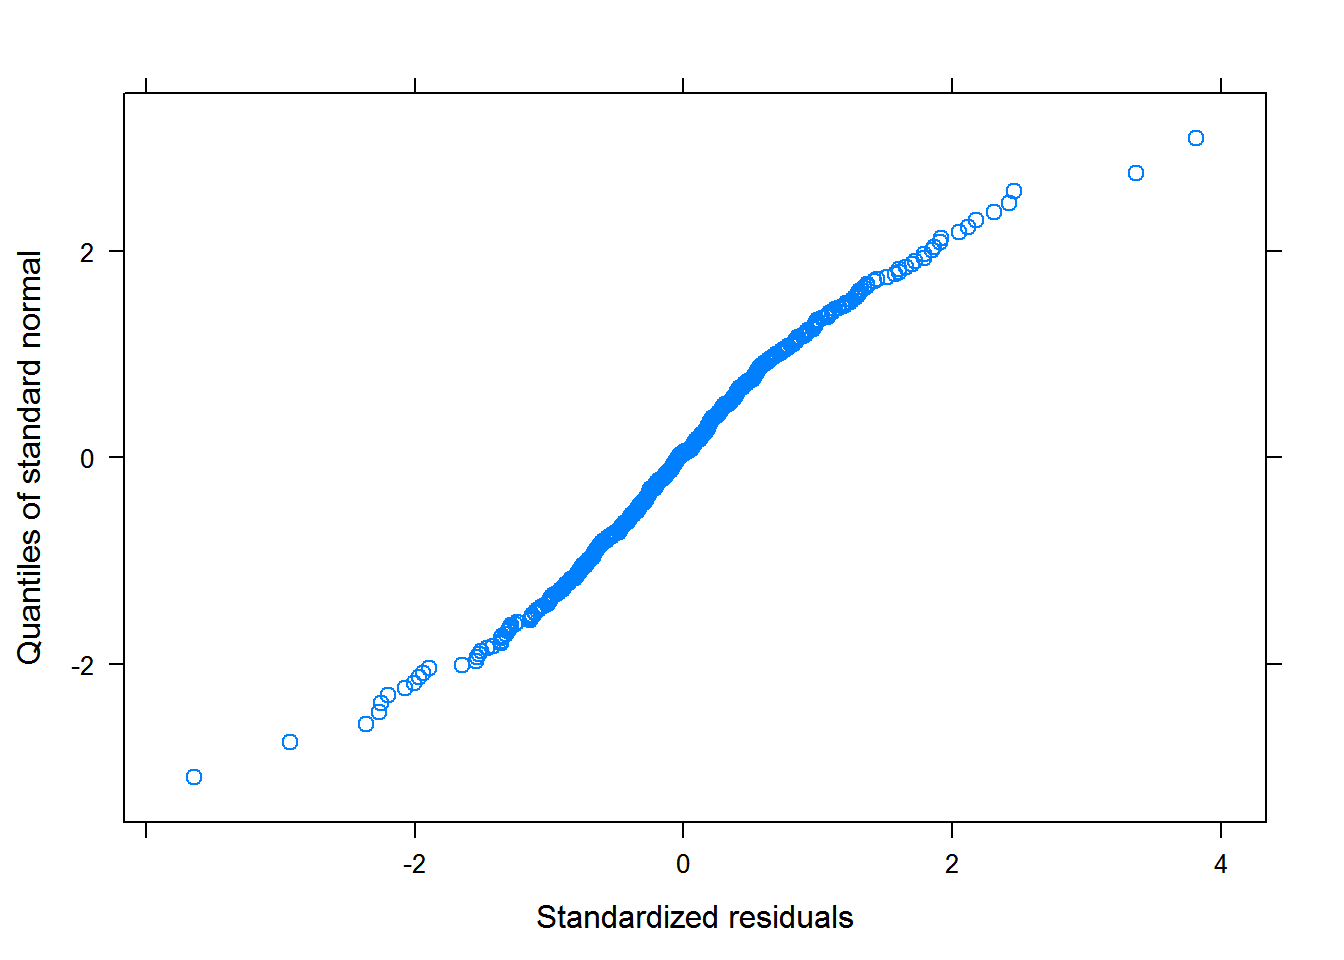
\includegraphics[width=0.9\linewidth]{images/ResidPlot3}
	\label{fig:ResidPlot3}
\end{figure}

This code will allow you to make QQ plots for each level of the random effects.  LME models assume that not only the within-cluster residuals are normally distributed, but that each level of the random effects are as well. Depending on the model, you can vary the level from 0, 1, 2 and so on
\begin{framed}
	\begin{verbatim}
	qqnorm(JS.roy1, ~ranef(.))

 # 	qqnorm(JS.roy1, ~ranef(.,levels=1)
	\end{verbatim}
\end{framed}
\begin{figure}[h!]
	\centering
	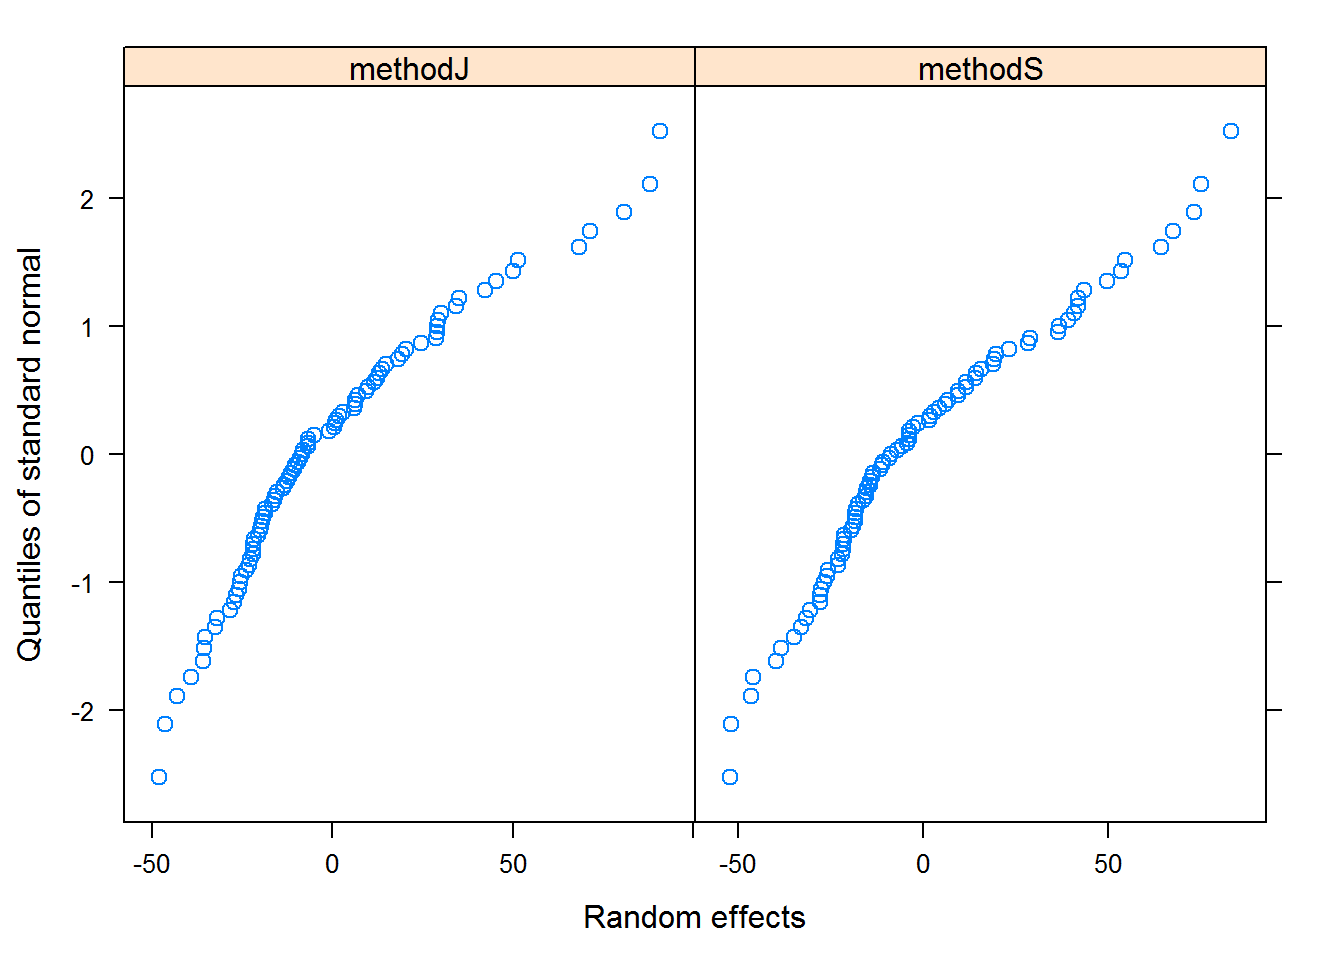
\includegraphics[width=0.9\linewidth]{images/ResidPlot2}
	\caption{}
	\label{fig:ResidPlot2}
\end{figure}


\section{Preliminaries: Useful R commands}


\texttt{vcov} returns the variance-covariance matrix of the main parameters of a fitted model object.
\begin{framed}
	\begin{verbatim}
	> vcov(JS.roy1)
	methodJ  methodS
	methodJ 11.01701  9.30105
	methodS  9.30105 11.75301
	\end{verbatim}
\end{framed}

\texttt{getVarCov} extract the variance-covariance matrix from a fitted model, such as a mixed-effects model.
\begin{framed}
	\begin{verbatim}
	> getVarCov(JS.roy1)
	Random effects variance covariance matrix
	methodJ methodS
	methodJ  923.98  785.23
	methodS  785.23  971.29
	Standard Deviations: 30.397 31.166 
	\end{verbatim}
\end{framed}	
\section{\texttt{coef.lme}}

The command \texttt{coef.lme} extract lmes coefficients


The estimated coefficients at level i are obtained by adding together the fixed effects estimates and the corresponding random effects estimates at grouping levels less or equal to i. The resulting estimates are returned as a data frame, with rows corresponding to groups and columns to coefficients. Optionally, the returned data frame may be augmented with covariates summarized over groups.
\begin{framed}
	\begin{verbatim}
	> JS.roy1 %>% coef %>% head(10)
	methodJ   methodS
	74  84.31724  91.08404
	36  91.54994  97.05548
	3   81.16581  96.48653
	62  92.09493  90.89073
	31  88.41411 103.38802
	42  95.56881 104.70922
	11 103.46092 111.33625
	41  94.97700 108.08384
	55  79.44762 110.02055
	17 101.53470 112.46964
	\end{verbatim}
\end{framed}
Suppose we refit the model, with a reduced data set ( for example, with subject 68 missing)

\begin{framed}
	\begin{verbatim}
	x=68
	datred <- dat[dat$subject !=x,]
	
	# datred is other 84 cases (504 observations)
	
	JS.roy1.red = lme(BP ~ method-1, 
	data = datred,
	random = list(subject=pdSymm(~ method-1)), 
	weights=varIdent(form=~1|method),
	correlation = corSymm(form=~1 | subject/repl), 
	method="ML")
	\end{verbatim}
\end{framed}

\begin{framed}
	\begin{verbatim}
	> JS.roy1.red %>% coef %>% dim
	[1] 84  2
	>
	> JS.roy1.red %>% coef %>% head(10)
	methodJ   methodS
	74  84.31425  90.89550
	36  91.54526  96.86813
	3   81.17663  96.36665
	62  92.07933  90.64629
	31  88.42473 103.27726
	42  95.57027 104.56000
	11 103.46071 111.18930
	41  94.98491 107.96791
	55  79.48324 110.02963
	17 101.53939 112.34591
	
	\end{verbatim}
\end{framed}




%============================================================================ %
\chapter{Using DFBETAs from LME Models to Assess Agreement}
	
	
	\citet{schab} examines the use and implementation of influence measures in LME models.
	
	Influence is understood to be the ability of a single or multiple data points, through their presences or absence in the data, to alter important aspects of the analysis, yield qualitatively 	different inferences, or violate assumptions of the statistical
	model \citep{schab}.
	
	Outliers are the most noteworthy data points in an analysis, and an objective of influence analysis is how influential they are,
	and the manner in which they are influential.
	
	\citet{schab} describes a simple procedure for quantifying influence.
	\begin{itemize}
		\item Firstly a model should be fitted to the data, and
		estimates of the parameters should be obtained.
		\item The second step is that either single or multiple data points, specifically outliers,
		should be omitted from the analysis, with the original parameter
		estimates being updated.
		\item  The final step of the procedure is comparing the 	sets of estimates computed from the entire and reduced data sets
		to determine whether the absence of observations changed the
		analysis.
	\end{itemize}
	   This is known as `\textit{leave one out} or \texttt{leave k
	out' analysis}.
	

		\section{Measures of Influence} %1.16
		
		The impact of an observation, or a case with multiple obverations, on a regression fitting can be determined by the difference between the estimated regression coefficient of a model with all observations and the estimated coefficient when the particular observation is deleted. The measure DFBETA is the studentized value of this difference.
		
		
		\subsection{Overall Influence}
		An overall influence statistic measures the change in the objective function being minimized. For example, in
		OLS regression, the residual sums of squares serves that purpose. In linear mixed models fit by
		\index{maximum likelihood} maximum likelihood (ML) or \index{restricted maximum likelihood} restricted maximum likelihood (REML), an overall influence measure is the \index{likelihood distance} likelihood distance [Cook and Weisberg ].
	%============================================================================= %
	\section{influence.ME}
	
	\textit{influence.ME} allows you to compute measures of influential data for mixed effects models generated by lme4.
	
	\textit{influence.ME} provides a collection of tools for detecting influential cases in generalized mixed effects models. It analyses models that were estimated using lme4. The basic rationale behind identifying influential data is that when iteratively single units are omitted from the data, models based on these data should not produce substantially different estimates. 
	
	To standardize the assessment of how influential a (single group of) observation(s) is, several measures of influence are common practice, such as DFBETAS and Cook's Distance. In addition, we provide a measure of percentage change of the fixed point estimates and a simple procedure to detect changing levels of significance.
\newpage
\section{Case Deletion Diagnostics} %1.6

\citet{CPJ} develops \index{case deletion diagnostics} case deletion diagnostics, in particular the equivalent of \index{Cook's distance} Cook's distance, for diagnosing influential observations when estimating the fixed effect parameters and variance components.

\subsection{Deletion Diagnostics}

Since the pioneering work of Cook in 1977, deletion measures have been applied to many statistical models for identifying influential observations.

Deletion diagnostics provide a means of assessing the influence of an observation (or groups of observations) on inference on the estimated parameters of LME models.

Data from single individuals, or a small group of subjects may influence non-linear mixed effects model selection. Diagnostics routinely applied in model building may identify such individuals, but these methods are not specifically designed for that purpose and are, therefore, not optimal. We describe two likelihood-based diagnostics for identifying individuals that can influence the choice between two competing models.

Case-deletion diagnostics provide a useful tool for identifying influential observations and outliers.

The computation of case deletion diagnostics in the classical model is made simple by the fact that estimates of $\beta$ and $\sigma^2$, which exclude the ith observation, can be computed without re-fitting the model. Such update formulas are available in the mixed model only if you assume that the covariance parameters are not affected by the removal of the observation in question. This is rarely a reasonable assumption.

\section{Effects on fitted and predicted values}
\begin{equation}
\hat{e_{i}}_{(U)} = y_{i} - x\hat{\beta}_{(U)}
\end{equation}

\subsection{Case Deletion Diagnostics for Mixed Models}

\citet{Christiansen} notes the case deletion diagnostics techniques have not been applied to linear mixed effects models and seeks to develop methodologies in that respect.

\citet{Christiansen} develops these techniques in the context of REML

%--------------------------------------------------------------------------%
\newpage
\section{Terminology for Case Deletion diagnostics} %1.8

\citet{preisser} describes two type of diagnostics. When the set consists of only one observation, the type is called
'observation-diagnostics'. For multiple observations, Preisser describes the diagnostics as 'cluster-deletion' diagnostics.	\section{Case Deletion Diagnostics}
	Case-deletion diagnostics provide a useful tool for identifying influential observations and outliers.
	
	The computation of case deletion diagnostics in the classical model is made simple by the fact that estimates of $\beta$ and $\sigma^2$, which exclude the ith observation, can be computed without re-fitting the model. Such update formulas are available in the mixed model only if you assume that the covariance parameters are not affected by the removal of the observation in question. This is rarely a reasonable assumption.
	
	Linear models for uncorrelated data have well established measures to gauge the influence of one or more
	observations on the analysis. For such models, closed-form update expressions allow efficient computations
	without refitting the model. 
	
	
	Since the pioneering work of Cook in 1977, deletion measures have been applied to many statistical models for identifying influential observations. Case-deletion diagnostics provide a useful tool for identifying influential observations and outliers.
	
	The key to making deletion diagnostics useable is the development of efficient computational formulas, allowing one to obtain the \index{case deletion diagnostics} case deletion diagnostics by making use of basic building blocks, computed only once for the full model.
	
	The computation of case deletion diagnostics in the classical model is made simple by the fact that estimates of $\beta$ and $\sigma^2$, which exclude the $i-$th observation, can be computed without re-fitting the model. %\subsection{Terminology for Case Deletion diagnostics} %1.8
	
	\citet{preisser} describes two type of diagnostics. When the set consists of only one observation, the type is called
	`\textit{observation-diagnostics}'. For multiple observations, Preisser describes the diagnostics as `\textit{cluster-deletion}' diagnostics. When applied to LME models, such update formulas are available only if one assumes that the covariance parameters are not affected by the removal of the observation in question. However, this is rarely a reasonable assumption.
	
	\subsection{Influence}
	\texttt{influence()} is the workhorse function of the influence.ME package. Based on a priorly estimated mixed effects regression model (estimated using lme4), the \texttt{influence()} function iteratively modifies the mixed effects model to neutralize the effect a grouped set of data has on the parameters, and which returns returns the fixed parameters of these iteratively modified models. These are used to compute measures of influential data.
	%============================================================================= %
	\section{Cooks's Distance}
	Cook's Distance is a measure indicating to what extent model parameters are influenced by (a set of) influential data on which the model is based. This function computes the Cook's distance based on the information returned by the estex() function.
	%============================================================================= %
	\section{DFBETAs}
	DFBETAS (standardized difference of the beta) is a measure that standardizes the absolute difference in parameter estimates between a (mixed effects) regression model based on a full set of data, and a model from which a (potentially influential) subset of data is removed. A value for DFBETAS is calculated for each parameter in the model separately. This function computes the DFBETAS based on the information returned by the estex() function.
	
	
	\subsection{Influence}
	
	Influence arises at two stages of the LME model. Firstly when $\mathbf{V}$ is estimated by $\hat{V}$, and subsequent
	estimations of the fixed and random regression coefficients $\mathbf{\beta}$ and $u$, given $\mathbf{\hat{V}}$.
	
	%- The Mahalanobis distance is a measure of the distance between a point P and a distribution D, introduced by P. C. Mahalanobis in 1936.
	4 It is a multi-dimensional generalization of the idea of measuring how many standard deviations away P is from the mean of D. 
	
	This distance is zero if P is at the mean of D, and grows as P moves away from the mean: Along each principal component axis, it measures the 
	number of standard deviations from P to the mean of D. If each of these axes is rescaled to have unit variance, then Mahalanobis distance corresponds to standard Euclidean distance in the transformed space. Mahalanobis distance is thus unitless and scale-invariant, and takes into account the correlations of the data set.
		%--------------------------------------------------------------------------%
		\newpage
		\subsubsection{Case Deletion Diagnostics}
		
		Since the pioneering work of Cook in 1977, deletion measures have been applied to many statistical models for identifying influential observations.
		
		Deletion diagnostics provide a means of assessing the influence of an observation (or groups of observations) on inference on the estimated parameters of LME models.
		
		Data from single individuals, or a small group of subjects may influence non-linear mixed effects model selection. Diagnostics routinely applied in model building may identify such individuals, but these methods are not specifically designed for that purpose and are, therefore, not optimal. We describe two likelihood-based diagnostics for identifying individuals that can influence the choice between two competing models.
		Case-deletion diagnostics provide a useful tool for identifying influential observations and outliers.
		
		The computation of case deletion diagnostics in the classical model is made simple by the fact that estimates of $\beta$ and $\sigma^2$, which exclude the ith observation, can be computed without re-fitting the model. Such update formulas are available in the mixed model only if you assume that the covariance parameters are not affected by the removal of the observation in question. This is rarely a reasonable assumption.
		
		\subsection{Terminology for Case Deletion diagnostics} %1.8
		
		\citet{preisser} describes two type of diagnostics. When the set consists of only one observation, the type is called
		'observation-diagnostics'. For multiple observations, Preisser describes the diagnostics as 'cluster-deletion' diagnostics.
	%============================================================================%
	\subsection*{Influence() - Description}
	\texttt{influence()} is the workhorse function of the \texttt{influence.ME} package. 
	
	
	Based on a priorly estimated mixed effects regression model (estimated using lme4), the \texttt{influence()} function iteratively 
	
	modifies the mixed effects model to neutralize the effect a grouped set of data has on the parameters, and which 
	
	returns returns the fixed parameters of these iteratively modified models. 
	
	These are used to compute measures of influential data.
	
	
	
	
	\subsection*{Usage}
	\begin{framed}
		\begin{verbatim}
		
		influence(model, group=NULL, select=NULL, obs=FALSE, 
		gf="single", count = FALSE, delete=TRUE, ...)
		\
		\end{verbatim}
	\end{framed}
	
	
	The \texttt{influence()} function was known as the \texttt{estex()} command in previous versions of the influence.ME pacakge
	%===========================================================================%
	%- http://support.sas.com/documentation/cdl/en/statug/63347/HTML/default/statug_reg_sect040.htm

	
	
	
	
	

	%-------------------------------------------------------------------------------------------------------------------------------------%
	\subsection{Influential Observations : DFBeta and DFBetas}
	% http://stats.stackexchange.com/questions/22161/how-to-read-cooks-distance-plots
	% Cook's distance refers to how far, on average, predicted y-values will move if the observation in question is dropped from the data set. 
	The dfbeta refers to how much a parameter estimate changes if the observation or case in question is dropped from the data set.  Cook's distance is presumably more important to you if you are doing predictive modeling, whereas dfbeta is more important in explanatory modeling.
	\subsection{DFBETA} %1.16.3
	DFBETAS (standardized difference of the beta) is a measure that standardizes the absolute difference in parameter estimates between a (mixed effects) regression model based on a full set of data, and a model from which a (potentially influential) subset of data is removed.
	%% -\subsection{DFBETA} %1.16.3
		\texttt{dfbeta()}
		
		
		The DFBETAS statistics are the scaled measures of the change in each parameter estimate and are calculated by deleting the th observation:
		
		where  is the th element of .
		In general, large values of DFBETAS indicate observations that are influential in estimating a given parameter. Belsley, Kuh, and Welsch (1980) recommend 2 as a general cutoff value to indicate influential observations and  as a size-adjusted cutoff.
		
	\begin{eqnarray}
	DFBETA_{a} &=& \hat{\beta} - \hat{\beta}_{(a)} \\
	&=& B(Y-Y_{\bar{a}}
	\end{eqnarray}
	In the case of method comparison studies, there are two covariates, and one can constru
	ct catterplots of the pairs of dfbeta values accordingly, both for LOO and LSO calculations. Furthermore 95\% confidence ellipse can be constructed around these scatterplots.
	Note that with k covariates, there will be $k+1$ dfbetas (the intercept,$\beta_0$, and 1 $\beta$ for each covariate). For example there would be 2 sets of of dfbeta, 510 valoues for each in the case of LOO, and 85 for LSO diagnostics.
	
	
	%-------------------------------------------------------------------------------------------------------------------------------------%
	
	\subsection{DFFITS} %1.16.1
	DFFITS is a statistical measured designed to a show how influential an observation is in a statistical model. 
	\begin{displaymath} DFFITS = {\widehat{y_i} -
		\widehat{y_{i(k)}} \over s_{(k)} \sqrt{h_{ii}}} \end{displaymath}
	It is closely related to the studentized residual. For the sake of brevity, we will concentrate on the Studentized Residuals.
	%===================================================================================== %
	\subsection{PRESS} %1.16.2
	The prediction residual sum of squares (PRESS) is an value associated with this calculation. When fitting linear models, PRESS can be used as a criterion for model selection, with smaller values indicating better model fits.
	\begin{equation}
	PRESS = \sum(y-y^{(k)})^2
	\end{equation}
	
	
	\begin{itemize}
		\item $e_{-Q} = y_{Q} - x_{Q}\hat{\beta}^{-Q}$
		\item $PRESS_{(U)} = y_{i} - x\hat{\beta}_{(U)}$
	\end{itemize}
	



%============================================================================= %
\section{Application of DFBETAs in MCS Analysis}


When in an MCS study. DFBetas can be used as a proxy measurement, allowing simple techniques to be used for assessing agreement.



\chapter{Model Diagnostics for MCS}

%-------------------------------------------------------------------------%
\begin{abstract}
Model diagnostic techniques, well established for classical models, have since been adapted for use with linear mixed effects models. However, diagnostic techniques for LME models are inevitably more difficult to implement, due to the increased complexity. \\ \bigskip


\citet{schab} describes the examination of model-data agreement as comprising several elements; \begin{itemize}
		\item residual analysis, 
		\item goodness of fit, 
		\item collinearity diagnostics
		\item influence analysis.
	\end{itemize} 
	
This chapter is comprised of two sections:
\begin{enumerate}
	\item Residual Diagnostics
	\item Influence Diagnostics
\end{enumerate}
\end{abstract}

%=============================================================================== %
\newpage
\section{Introduction}
In statistical modelling, the process of model validation is a critical step, but also a step that is too often overlooked. A very simple procedure is to examine well known
metrics, such as the AIC and $R^2$ measures. However, using a small handful of simple measures and methods is insufficient to properly assess the quality of a fitted model. To do so properly, a full and comprehensive
analysis that tests of all of the assumptions, as far as possible, must be carried out. 

A statistical model, whether of the fixed-effects or mixed-effects variety, represents how you think your data were generated. Following model specification and estimation, it is of interest to explore the model-data
agreement by raising pertinent questions. Further to the analysis of residuals, \citet{schab} recommends the examination of the following questions.
\begin{itemize}
	\item Does the model-data agreement support the model assumptions?
	\item Should model components be refined, and if so, which components? For example, should certain explanatory variables
	be added or removed, and is the covariance of the observations properly specified?
	\item Are the results sensitive to model and/or data? Are individual data points or groups of cases particularly
	influential on the analysis?
\end{itemize}
\newpage

\section{Introduction to Influence analysis} %1.7
 Model diagnostic techniques determine whether or not the distributional assumptions are satisfied, and to assess the influence of unusual observations. In classical linear models model diagnostics have been become a required part of any statistical analysis, and the methods are commonly available in statistical packages and standard textbooks on applied regression. However it has been noted by several papers that model diagnostics do not often accompany LME model analyses.
For linear models for uncorrelated data, it is not necessary to refit the model after removing a data point in order to measure the impact of an observation on the model. The change in fixed effect estimates, residuals, residual sums of squares, and the variance-covariance matrix of the fixed effects can be computed based on the fit to the full data alone. By contrast, in mixed models several important complications arise. Data points can affect not only the fixed effects but also the covariance parameter estimates on which the fixed-effects estimates depend. 

\subsection{What is Influence} %1.1.5


Broadly defined, influence is understood as the ability of a single or multiple data points, through their presence or absence in the data, to alter important aspects of the analysis, yield qualitatively different inferences, or violate assumptions of the statistical model. The goal of influence analysis is not primarily to mark data points for deletion so that a better model fit can be achieved for the reduced data, although this might be a result of influence analysis \citep{schabenberger}.


\subsection{Importance of Influence}
The influence of an observation can be thought of in terms of how much the predicted values for other observations would differ if the observation in question were not included in the model fit.
Likelihood based estimation methods, such as ML and REML, are sensitive to unusual observations. Influence diagnostics are formal techniques that assess the influence of observations on parameter estimates for $\beta$ and $\theta$. A common technique is to refit the model with an observation or group of observations omitted. The basic procedure for quantifying influence is simple as follows:


\begin{enumerate}
	\item Fit the model to the data and obtain estimates of all parameters.
	\item Remove one or more data points from the analysis and compute updated estimates of model parameters.
	\item Based on full- and reduced-data estimates, contrast quantities of interest to determine how the absence of the observations changes the analysis.
\end{enumerate}
\subsection{Measures of Influence} 
% DFBETA
% DFFITS
% PRESS
The impact of an observation on a regression fitting can be determined by the difference between the estimated regression coefficient of a model with all observations and the estimated coefficient when the particular observation is deleted. DFBETA and DFFITS are well known measures of influenc. The measure DFBETA is the studentized value of this difference.	DFFITS is a statistical measured designed to a show how influential an observation is in a statistical model. DFFITS is closely related to the studentized residual.

\begin{eqnarray}
DFBETA_{a} &=& \hat{\beta} - \hat{\beta}_{(a)} \\
&=& B(Y-Y_{\bar{a}}
\\ DFFITS = {\widehat{y_i} -
	\widehat{y_{i(k)}} \over s_{(k)} \sqrt{h_{ii}}} 
\end{eqnarray}

The prediction residual sum of squares (PRESS) is an value associated with this calculation. When fitting linear models, PRESS can be used as a criterion for model selection, with smaller values indicating better model fits.
\begin{displaymath}
PRESS = \sum(y-y^{(k)})^2
\end{displaymath}
%	
%	\begin{itemize}
%		\item $e_{-Q} = y_{Q} - x_{Q}\hat{\beta}^{-Q}$
%		\item $PRESS_{(U)} = y_{i} - x\hat{\beta}_{(U)}$
%	\end{itemize}
%	
\subsection{DFBETAs}
The measure that measures how much impact each observation has on a particular predictor is DFBETAs The DFBETA for a predictor and for a particular observation is the difference between the regression coefficient calculated for all of the data and the regression coefficient calculated with the observation deleted, scaled by the standard error calculated with the observation deleted.

DFBETA is a measure found for each observation in a dataset. The DFBETA for a 
particular observation is the difference between the regression coefficient for an included variable calculated for all of the data and the regression coefficient calculated with the observation deleted, scaled by the standard error calculated with the 
observation deleted. 

The cut-off value for DFBETAs is $\frac{2}{\sqrt{n}}$, where n is the number of observations. 
However, another cut-off is to look for observations with a value greater than 1.00. Here cutoff means, 
“this observation could be overly influential on the estimated coefficient.” 
%==========================================================================%
%WIKIPEDIA
\subsubsection{DFFITS}
DFFITS is a diagnostic meant to show how influential a point is in a statistical regression. It was proposed in 1980. It is defined as the change ("DFFIT"), in the predicted value for a point, obtained when that point is left out of the regression, "Studentized" by dividing by the estimated standard deviation of the fit at that point:
\[ \mbox{DFFITS} = {\widehat{y_i} - \widehat{y_{i(i)}} \over s_{(i)} \sqrt{h_{ii}}}\]

\subsubsection{DFbetas for Blood Data}
\begin{framed}
	\begin{verbatim}
	plot(JS.roy1.dfbeta$all.res1[1:255],JS.roy1.dfbeta$all.res2[256:510],
	pch=16,col="blue")
	abline(v=JS.roy1.dfbeta$all.res1[256],col="red")
	abline(h=JS.roy1.dfbeta$all.res2[1],col="red")
	\end{verbatim}
\end{framed}
\begin{figure}
	\centering
	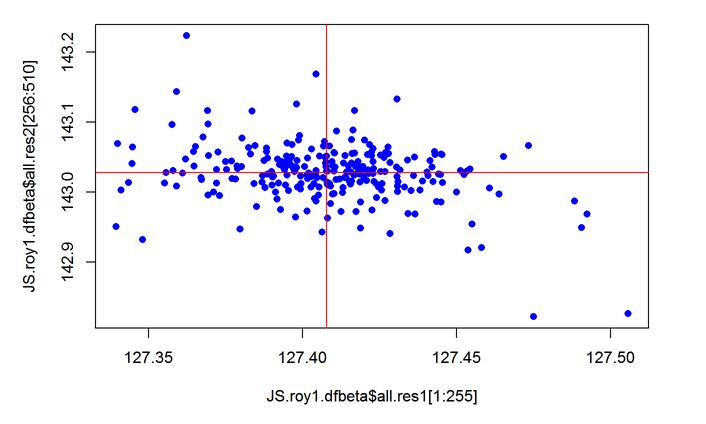
\includegraphics[width=0.7\linewidth]{images/dfbetas-JS-ROY}
	\caption{}
	\label{fig:dfbetas-JS-ROY}
\end{figure}







%---------------------------------------------------------------------------%
%---------------------------------------------------------------------------%
\newpage
\subsection{Local Influence Analysis}



% - \citet{Beckman}
Beckman, Nachtsheim and Cook (1987)  applied the \index{local influence}local influence method of Cook (1986) to the analysis of the linear mixed model.

While the concept of influence analysis is straightforward, implementation in mixed models is more complex. Update formulae for fixed effects models are available only when the covariance parameters are assumed to be known.

If the global measure suggests that the points in $U$ are influential, the nature of that influence should be determined. In particular, the points in $U$ can affect the following

\begin{itemize}
	\item the estimates of fixed effects,
	\item the estimates of the precision of the fixed effects,
	\item the estimates of the covariance parameters,
	\item the estimates of the precision of the covariance parameters,
	\item fitted and predicted values.
\end{itemize}


\newpage
\subsection{Likelihood Distances}

The \index{likelihood distance} likelihood distance is a global summary measure that expresses the joint influence of the subsets of observations, $U$, on all parameters in $\phi$ that were subject to updating. For classical linear models, the implementation of influence analysis is straightforward. \citet{schab} points out the likelihood distance gives the amount by which the log-likelihood of the model fitted from the full data changes if one were
to estimate the model from a reduced-data estimates. Importantly $LD(\psi_{(U)})$ is not the log-likelihood obtained by fitting the model to the reduced data set. It is obtained by evaluating the likelihood function based on the full data set (containing all $n$ observations) at the reduced-data estimates.


%---------------------------------------------------------- %
%Likelihood Displacement.
\[  LD(\boldsymbol{(U)})= 2[l\boldsymbol{\hat{(\phi)}} - l\boldsymbol{\hat{\phi}_\omega} ] \]
\[  RLD(\boldsymbol{(U)})= 2[ l_R\boldsymbol{\hat{(\phi)}} - l_R\boldsymbol{\hat{(\phi)}_\omega} ] \]
%	Large values indicate that $\boldsymbol{\hat{\theta}}$ and $\boldsymbol{\hat{\theta}_\omega}$ differ considerably.


An overall influence statistic measures the change in the objective function being minimized. For example, in
OLS regression, the residual sums of squares serves that purpose. In linear mixed models fit by
\index{maximum likelihood} maximum likelihood (ML) or \index{restricted maximum likelihood} restricted maximum likelihood (REML), an overall influence measure is the \index{likelihood distance} likelihood distance \citep{cook}. In LME models, fitted by either ML or REML, an important overall
 influence measure is the likelihood distance \citep{cook82}. The  procedure requires the calculation of the full data estimates
 $\hat{\psi}$ and estimates based on the reduced data set  $\hat{\psi}_{(U)}$. The likelihood distance is given by
 determining
 
 
 \begin{eqnarray}
 LD_{(U)} &=& 2\{l(\hat{\psi}) - l( \hat{\psi}_{(U)}) \}\\
 RLD_{(U)} &=& 2\{l_{R}(\hat{\psi}) - l_{R}(\hat{\psi}_{(U)})\}
 \end{eqnarray}
%----schabenberger page 8
For classical linear models, the implementation of influence analysis is straightforward.
However, for LME models, the problem is more complex. Update formulas for the fixed effects are available only when the covariance parameters are assumed to be known. A measure of total influence requires updates of all model parameters. This can only be achieved in general is by omitting observations or cases, then refitting the model. This is a very simplistic approach, and computationally expensive.

\citet{west} examines a group of methods that examine various aspects of influence diagnostics for LME models.
For overall influence, the most common approaches are the \textit{likelihood distance} and the \textit{restricted likelihood distance}.

\subsubsection{The \texttt{logLik} Function}
\texttt{logLik.lme} returns the log-likelihood value of the linear mixed-effects model represented by object evaluated at the estimated coefficients. It is also possible to determine the restricted log-likelihood, if relevant, using this function. For the Blood Data Example,  the loglikelihood of the JS.roy1 model can be computed as follows.
\begin{framed}
\begin{verbatim}
> logLik(JS.roy1)
'log Lik.' -2030.736 (df=8)
\end{verbatim}
\end{framed}
%======================================================================================= %
\newpage
\subsection{Cook's Distance}
\citet{CPJ} develops \index{case deletion diagnostics} case deletion diagnostics, in particular the equivalent of \index{Cook's distance} Cook's distance, a well-known metric, for diagnosing influential observations when estimating the fixed effect parameters and variance components. Deletion diagnostics provide a means of assessing the influence of an observation (or groups of observations) on inference on the estimated parameters of LME models. 
%We shall provide a fuller discussion of Cook's distance in due course.
Cook's Distance is a good measure of the influence of an observation that is a measure of aggregate impact of each observation on the group of regression coefficients, as well as the group of fitted values.
%Cook's Distance is proportional to the sum of the squared differences between predictions made with all observations in the analysis and predictions made leaving out the observation in question. 
If the predictions are the same with or without the observation in question, then the observation has no influence on the regression model. If the predictions differ greatly when the observation is not included in the analysis, then the observation is influential.

%======================================================================================= %
\newpage
% Hence the name deletion diagnostics and case-deletion diagnostics. 
\subsubsection{Cook's Distance for Blood Data}
\begin{figure}[h!]
	\centering
	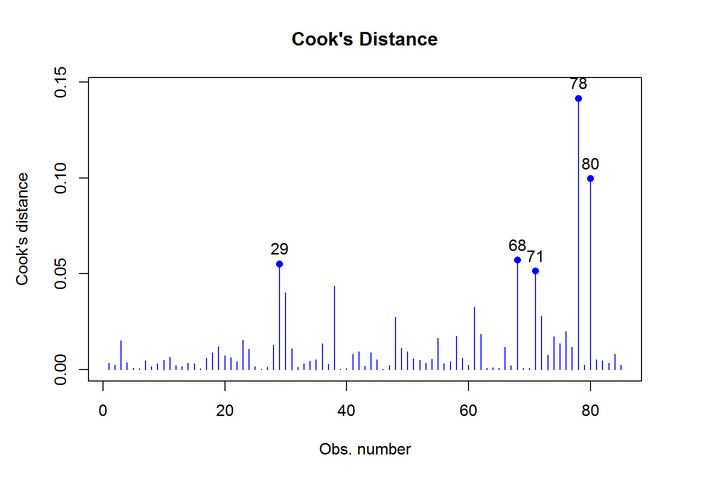
\includegraphics[width=0.9\linewidth]{images/CooksDistancePlot-JS-Roy}
%	\caption{}
%	\label{fig:CooksDistancePlot-JS-Roy}
\end{figure}


\newpage
\subsection{Deviance}
In statistics, deviance is a quality of fit statistic for a model that is often used for statistical hypothesis testing. It is a generalization of the idea of using the sum of squares of residuals in ordinary least squares to cases where model-fitting is achieved by maximum likelihood.

%-----------------------------------%


\bibliography{DB-txfrbib}
\end{document}
%================================================================================ %
